\documentclass[a4paper]{ujarticle}

\usepackage{mymacro}
\usepackage{graphicx}
\usepackage[dvipdfmx]{color}
\usepackage{xcolor}
\usepackage{here} % \begin{figure}[H]
\usepackage{ascmac} % \boxnote ほか
\usepackage{listings, jlisting}
%% -- \url link
\usepackage[linkcolor=black]{hyperref}
\usepackage[hyperrefcolorlinks,os=win]{menukeys}
\usepackage{pxjahyper}
%% --
\lstset{language=c,
  breaklines = true,
  linewidth=\textwidth,
  xleftmargin=20pt,
  xrightmargin=20pt,
  basicstyle={\footnotesize\ttfamily},
  identifierstyle={\footnotesize\ttfamily},
  commentstyle={\footnotesize\ttfamily},
  keywordstyle={\footnotesize\ttfamily},
  ndkeywordstyle={\footnotesize\ttfamily},
  stringstyle={\footnotesize\ttfamily},
  classoffset=1,
  frame=tRBl,
  framesep=5pt,
  showstringspaces=false,
  numbers=left,
  stepnumber=1,
  tabsize=4
}
%%
\begin{document}

\thispagestyle{empty}
%!TEX root = ./NCVC.tex

\vspace*{4zh}
\begin{figure}[H]
\centering

\includegraphics[scale=1.2]{logo.png}
\end{figure}

\vspace*{3zh}
\begin{center}
    \rule{6cm}{0.2zw}\\[-0.5zh]
    \rule{5cm}{0.1zw}\\[-0.5zh]
    \rule{4cm}{0.05zw}\\[1zh]
    {\Large \textbf{NCVC解説書}}\\
    \rule{4cm}{0.05zw}\\[-0.5zh]
    \rule{5cm}{0.1zw}\\[-0.5zh]
    \rule{6cm}{0.2zw}

    \vspace*{8cm}
    NCVC Ver0.14.42 用\\
    2005 年 10 月 初版
\end{center}

\newpage

\setcounter{page}{0}
\thispagestyle{empty}
{\small \tableofcontents}

\vspace*{2zh}
\begin{center}
\begin{minipage}{10cm}
\begin{screen}
NCVC(NC Viewer and Converter)は眞柄賢一の著作物です.
Jw\_cad for Windows は Jiro Shimizu \& Yoshifumi Tanaka 両氏の著作物です.
その他本解説書に記載された製品名・会社名などは,各社の商標または登録商標です.
各権利を侵害する行為は堅くお断りします.
本解説書に掲載されている操作等は各自の責任で行って下さい.
著者は一切責任を持ちません.  
\end{screen}
\end{minipage}
\end{center}
\newpage

%!TEX root = ./NCVC.tex

\mysection{はじめに}

\vspace*{2zh}
 NCVC(NC Viewer and Converter)はCAMソフトです.
主にCAD情報からNC工作機械を動かすためのGコードを生成するアプリケーションです.
NCVCにCAD(作図)機能は付いていません.
作図は別途CADソフトで行って下さい.
CADソフトは Jw\_cad for Windows (以降 Jw\_cad と略記)を推奨しますが,
以下の条件に当てはまるCADならNCVCの入力源としてそのまま使えます.

\begin{itemize}
    \item R12形式のDXFが出力可能なもの
    \item DXFにレイヤ情報(レイヤ名)が出力できるもの
\end{itemize}

 ほとんどのCADが当てはまると思います.
普段使い慣れたCADソフトをご使用下さい.
逆に言うとNCVCを使うためにわざわざ新たなCADの操作方法を覚える必要が無いということです.
以降本解説書でのCAD操作は Jw\_cad をベースに解説します.

 残念ながらCADを使ったことが無いという方,本解説書ではCADの使用を前提にしています.
上記条件を満たしていればドロー系ソフトでもかまいませんが,正確な作図が要求されます.
まずはCADでの作図方法を習得して下さい.

 もう1つ,NCVCにはGコードのシミュレーション機能がありますが,
冒頭で述べたとおりNCVCはGコードの生成を主な目的としています.
全てのGコードには対応していませんので,サポートされるGコードは付録の対応Gコード一覧を参照して下さい.
また,シミュレーション結果と工作機械の動作が必ず一致するとも限りません.
実際の加工にはくれぐれもご注意下さい.

\vspace*{2zh}
\begin{center}
\begin{minipage}{10cm}
\begin{screen}
NCVC(NC Viewer and Converter)は眞柄賢一の著作物です.
Jw\_cad for Windows は Jiro Shimizu \& Yoshifumi Tanaka 両氏の著作物です.
その他本解説書に記載された製品名・会社名などは,各社の商標または登録商標です.
各権利を侵害する行為は堅くお断りします.
本解説書に掲載されている操作等は各自の責任で行って下さい.
著者は一切責任を持ちません.  
\end{screen}
\end{minipage}
\end{center}

\vspace*{2zh}
\begin{boxnote}
 この解説書は一太郎で書いた初代NCVC解説書を \TeX で書き直したものです.
古い表記がありますが,適宜置き換えてください.
関連書籍を出版しているので,原則そちらを参照してください.
\begin{center}
\url{https://shop.ohmsha.co.jp/shopdetail/000000005207/}
\end{center}
少なくとも書籍が絶版になるまでは,内容が更新されることはありません.
\end{boxnote}
\newpage

%!TEX root = ../NCVC.tex

\mysection{基本編}

\subsection{CADでの作図}

\begin{minipage}[t]{0.4\textwidth}
 まずは基本的な加工を行うための基本的な作図方法を解説します.
図\ref{fig:sample1.jww} のような図形を書きましょう.
切削対象(ワーク)を示す矩形と,その矩形左下に円を1つ.
「NCVC」という文字は,線をつなぎ合わせたデータです.
\end{minipage}
\begin{minipage}[t]{0.6\textwidth}
\vspace*{-2zh}
\begin{figure}[H]
\centering
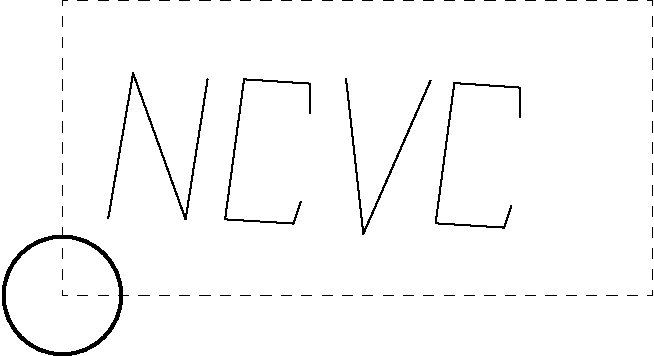
\includegraphics[scale=0.8]{No1/fig/sample1.pdf}
\caption{サンプル図形}
\label{fig:sample1.jww}
\end{figure}
\end{minipage}

\vspace*{2zh}
 NCVCはCADでの作図情報を全て読み込むのではなく,
特定のレイヤ情報を元に作図データを読み込みます.
CADでの作図において必要とされる補助線や寸法線等が加工データには必要なく,
これらを選別するための仕様です.

 その選別方法は『必要なレイヤに名前を付ける』こと.
図\ref{fig:sampleLayer.png} は図\ref{fig:sample1.jww} のレイヤ情報ですが,
0番レイヤに「ORIGIN」という名前,
1番レイヤに「CAM\_LINE」という名前を付けています.
それぞれ機械原点と切削軌跡を示し,この2つのレイヤは必須です
\footnote{実は機械原点レイヤは必須ではありません.詳細は【穴加工】の節で解説しています.}.
機械原点レイヤには工作機械のXY原点を示す円を1つだけ作図.
大きさは任意ですが,円の中心がXYの原点となります.
切削軌跡 CAM\_LINE レイヤには刃物のパス,
すなわち削りたい図形を書きます.
他,ワーク矩形を示す補助線等は別のレイヤに書きます.
レイヤに名前を付ける方法は,それぞれのCAD操作に準拠して下さい.
なお,全てのデータにおいて線種,線色は関係ありません.

\vspace*{1zh}
\begin{figure}[H]
\centering
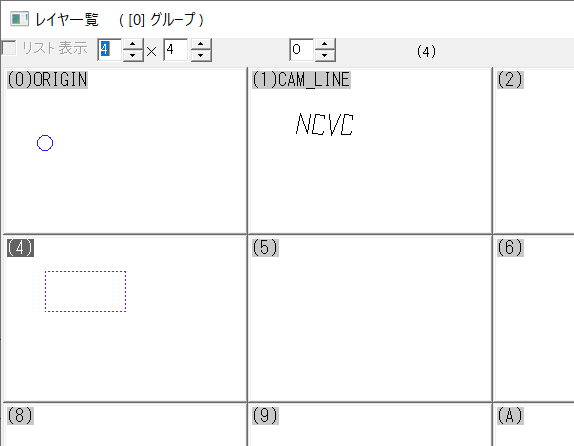
\includegraphics{No1/fig/sampleLayer.png}
\caption{レイヤ一覧}
\label{fig:sampleLayer.png}
\end{figure}

 作図が終わればCADデータをDXF形式で保存します
\footnote{
    Jw\_cadの場合,DXF形式で保存する必要はありません.NCVCはJWW形式を直接読み込むことが可能です.
    詳細は【パワーユーザ編】の【アドイン作成のすすめ】を参照して下さい.
}.
NCVCにCADデータを読み込ませるためDXF形式で保存する必要がありますが,
多くの場合,DXF形式で保存するとそのCAD独自のデータが失われるため,
使用しているCAD独自の形式でも保存しておきましょう.

\subsection{CADデータの読み込み}

\begin{minipage}[t]{0.5\textwidth}
 NCVCでDXF形式のCADデータを読み込みます.
が,その前に確認.
NCVCの \menu{オプション>DXF関連の設定} をクリックし,
NCVCが読み込むレイヤ名を設定して下さい.
デフォルトで先ほど設定した値になっていると思います.
基本編では[従来互換]のみ解説しますので,図\ref{fig:NCVCsetup.png} の通り設定して下さい.
この値は任意です.CAD側の設定と合わせて下さい.
無事読み込めると原点を示す十字(大きさは原点円の直径)と切削対象のパスが表示されます.
原点レイヤと切削レイヤ以外に作図した情報,
例えば,図\ref{fig:sampleLayer.png} の4番レイヤに書いたワークを表す矩形は読み込まれません(図\ref{fig:NCVCread.png}).
CADでの線種・線色は無視され,NCVCの設定に基づき表示されます.
詳細はリファレンスの表示属性を参照してください.
\end{minipage}
\begin{minipage}[t]{0.5\textwidth}
\vspace*{-2zh}
\begin{figure}[H]
\centering
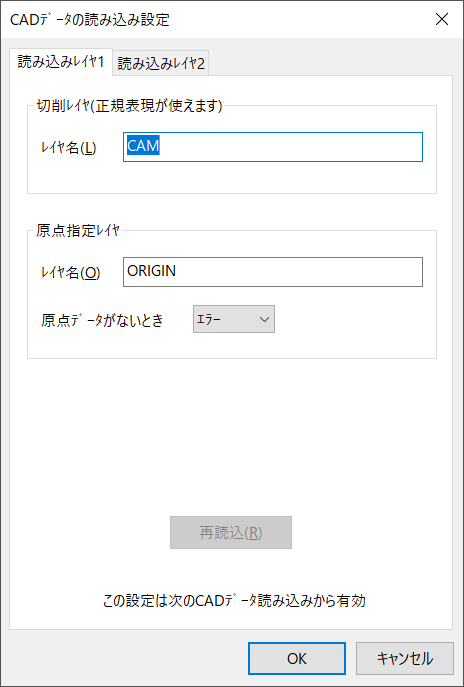
\includegraphics[scale=0.8]{No1/fig/NCVCsetup.png}
\caption{読み込みレイヤ設定}
\label{fig:NCVCsetup.png}
\end{figure}
\end{minipage}

\begin{figure}[H]
\centering
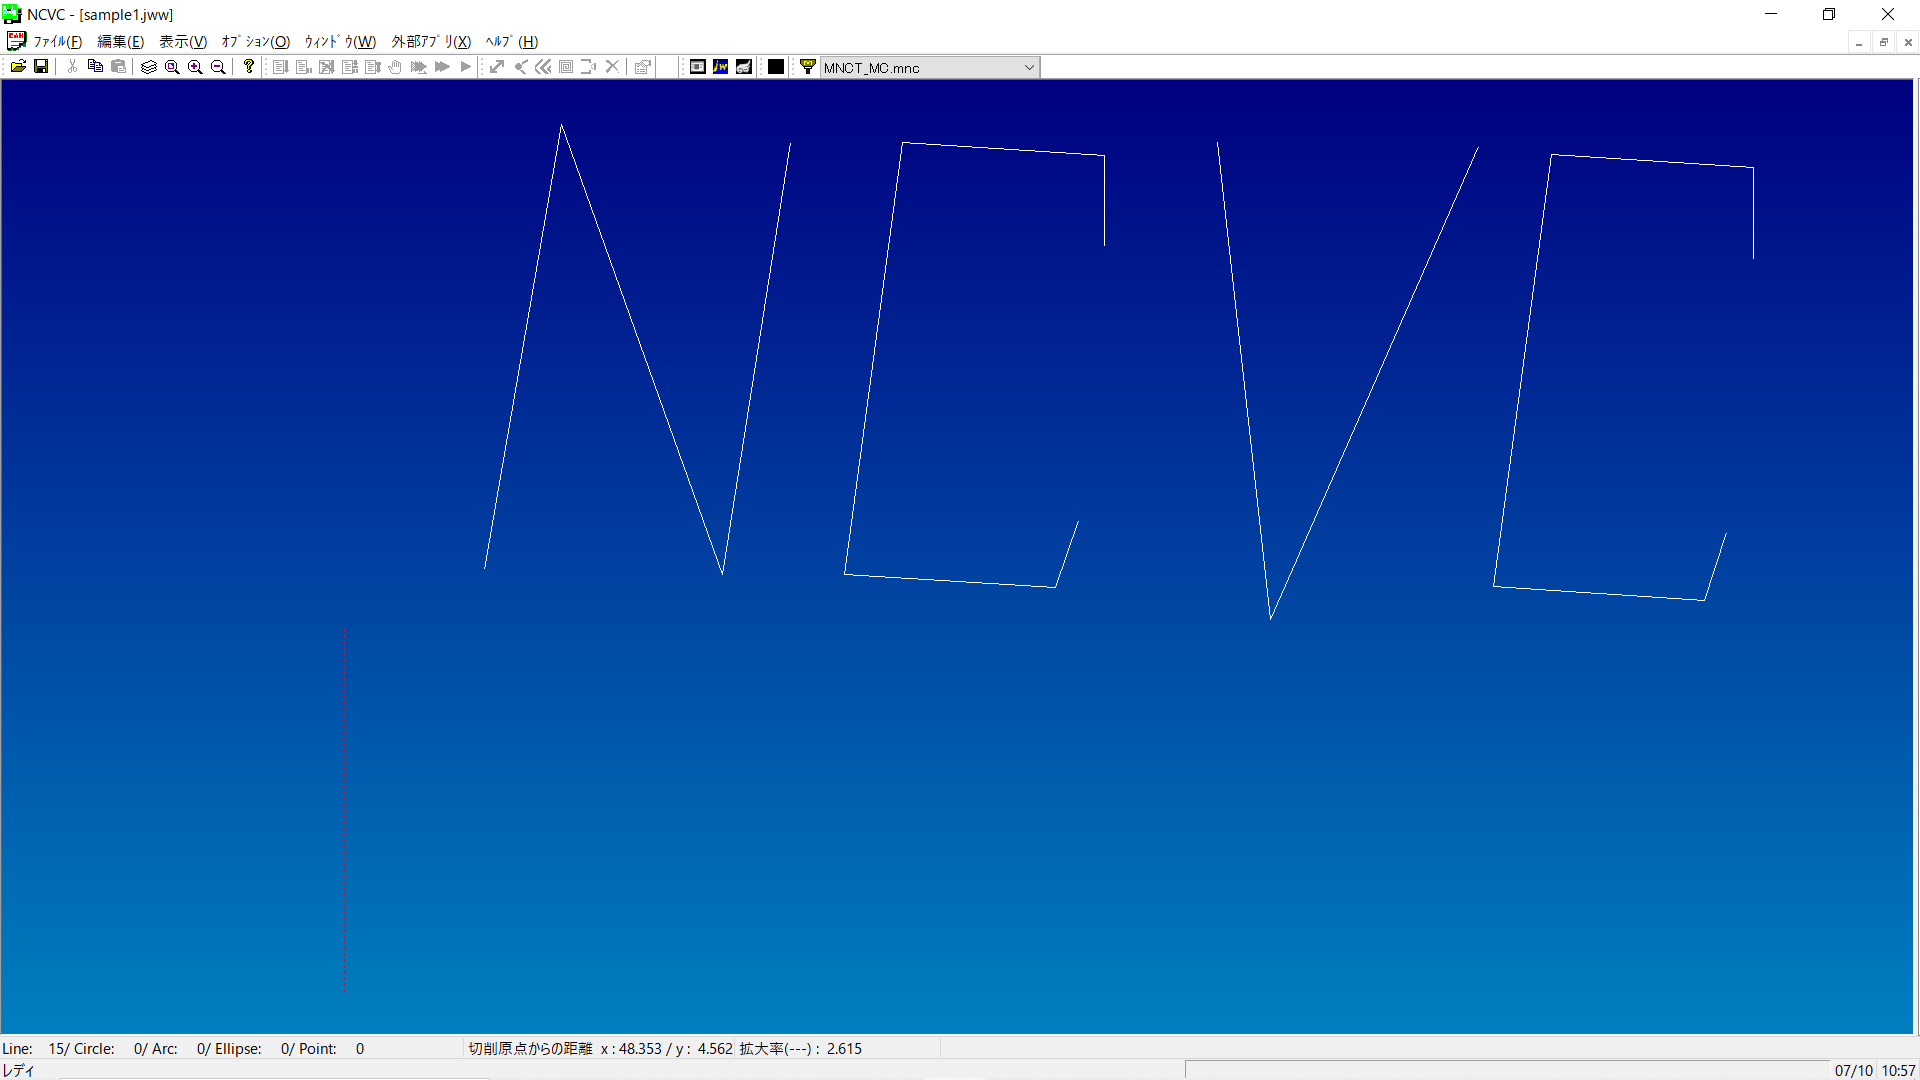
\includegraphics[scale=0.4]{No1/fig/NCVCread.png}
\caption{CADデータの読み込み}
\label{fig:NCVCread.png}
\end{figure}

\subsection{加工条件の設定}

 いよいよCADデータからGコードを生成するわけですが,ご覧の通り読み込んだCADデータは2次元です.
工作機械のZ軸方向の移動はどうやって制御するのでしょうか?
答えは[加工条件]の中にあります.
\menu{オプション>切削パラメータの設定} をクリックし,条件ファイル(nciファイル)を選択します.
標準で用意されている[Init.nci]の設定を変更しましょう.

 条件ファイルを選択すると図\ref{fig:init.nci.png} のダイアログが表示されます.
ここで重要なのが切削原点(G92)のZ値とR点,切り込みパラメータの3つです.

 図\ref{fig:XZ-crop.pdf} は工作機械を正面から見た図,上下にZ軸,左右にX軸です.
ワークをセットしたあと,ワーク平面を基準にZセンサー等でZ軸の位置決めを行います.
これを切削原点(G92)のZ値とします.
Zセンサーの厚みが100mmなら100と入力です.
センサーでの調整後,好みの位置に移動させてもかまいません.
無論そのときは移動した座標値を入力して下さい.

 次に切り込みですが,イメージ通り.ワークに何ミリ切り込むかという設定です.
最後にR点ですが,これは次の切削領域,この例で言うと``\,N\,''を削って``\,C\,''に移動するときのZ値を指定します.
Z軸の初期位置(原点)で移動してもかまわないのですが,初期位置は高く設定する傾向があるため,効率よく移動できる下限値と考えて下さい.
この設定ではワーク平面上空1mmの所で刃物が次の切削領域へ高速移動します.

 ワーク平面を基準に値を選びましたが,Zセンサー調整後の位置を基準,
すなわち,ワーク上空10mmの位置をZ軸の原点(G92Zをゼロ)としたとき,この例ではR点が-9mm,切り込みは-12mmとなります.
意味は同じですから各自の好みや考えやすい方で指示して下さい.

 他,主軸回転数や送り速度など,ワーク材質に合わせて設定します.

\begin{minipage}{0.5\textwidth}
\begin{figure}[H]
\centering
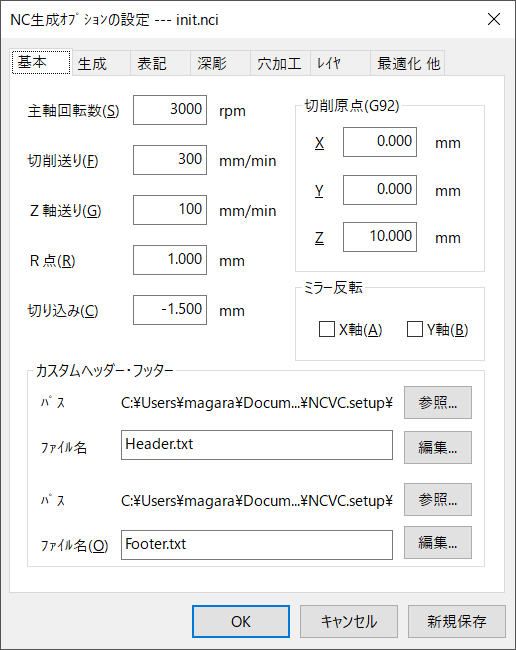
\includegraphics[scale=0.7]{No1/fig/init.nci.png}
\caption{加工条件の設定}
\label{fig:init.nci.png}
\end{figure}
\end{minipage}
\begin{minipage}{0.5\textwidth}
\begin{figure}[H]
\centering
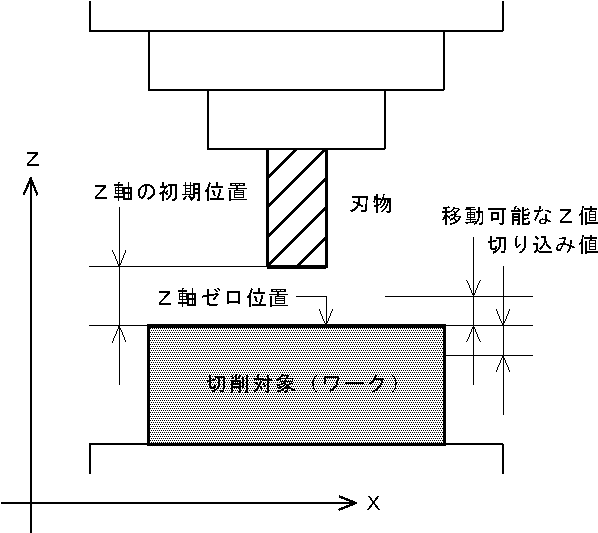
\includegraphics[scale=0.8]{No1/fig/XZ-crop.pdf}
\caption{Z軸における各パラメータの関係}
\label{fig:XZ-crop.pdf}
\end{figure}
\end{minipage}

\subsection{Gコードの生成}

\begin{minipage}[t]{0.5\textwidth}
 加工条件の設定ができればあとはNCVCの仕事.
\menu{ファイル>NCデータへの変換>単一条件(従来互換)} をクリック.
出力ファイル名(自動設定)と条件ファイルを指定(図\ref{fig:make.png})し,OKをクリックすれば
\end{minipage}
\begin{minipage}[t]{0.5\textwidth}
\vspace*{-2zh}
\begin{figure}[H]
\centering
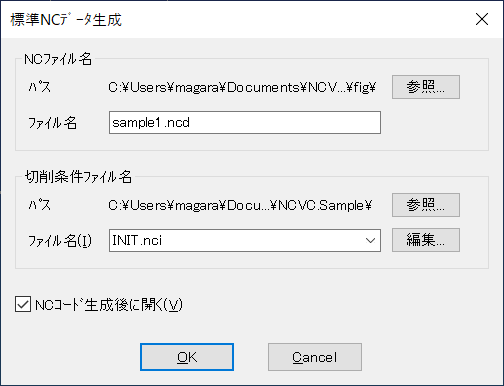
\includegraphics[scale=0.7]{No1/fig/make.png}
\caption{Gコードの出力と条件ファイルの指示}
\label{fig:make.png}
\end{figure}
\end{minipage}

\vspace*{2zh}
 おめでとうございます!見事Gコードが生成できました.
図\ref{fig:make.png} で[NC生成後に開く]にチェックが入っていると,即座に結果を確認することが出来ます.
図\ref{fig:sim.png} にGコードのシミュレーション結果を示します.

\begin{figure}[H]
\centering
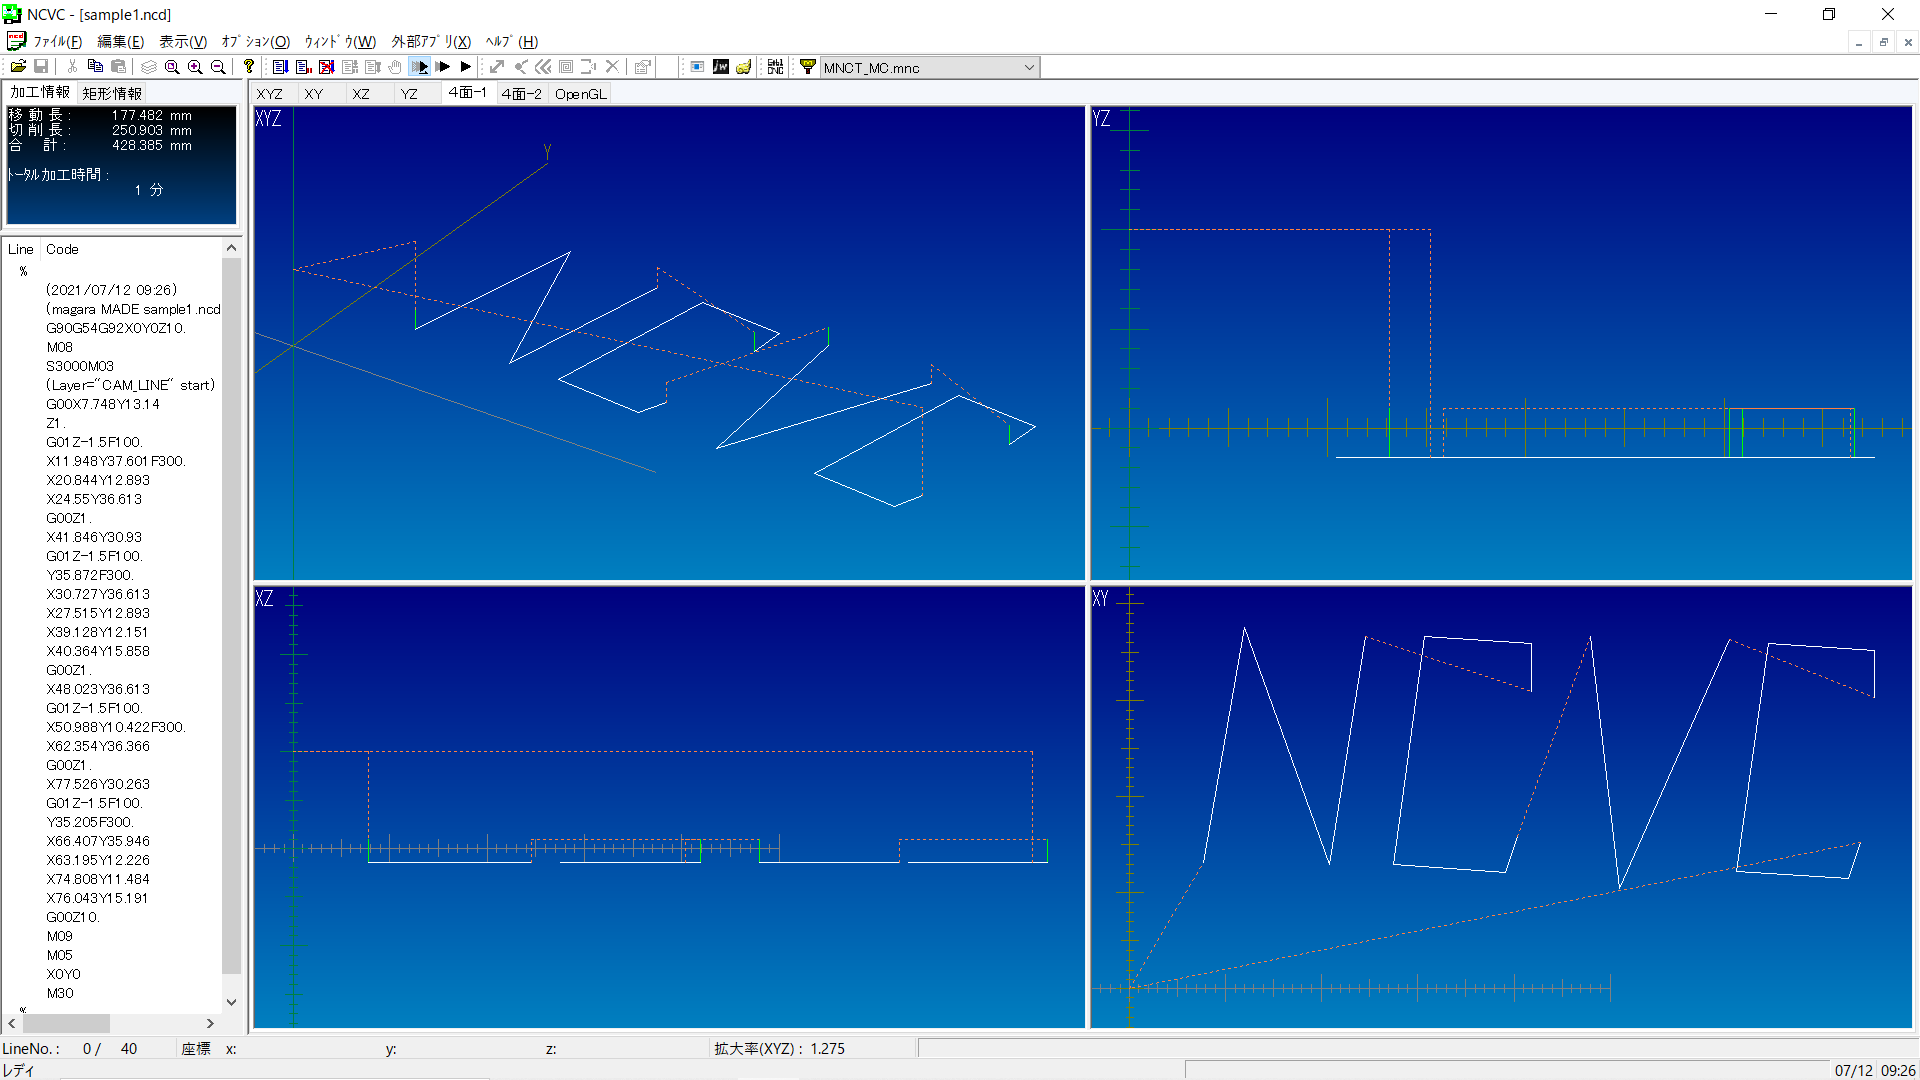
\includegraphics[scale=0.4]{No1/fig/sim.png}
\caption{Gコードシミュレーション画面}
\label{fig:sim.png}
\end{figure}

\vspace*{2zh}
\begin{itembox}[l]{ここまでの【まとめ】}
(1) CADでの操作
\begin{itemize}
\item 工作機械のXY原点を示す円を原点レイヤに作図
\item 刃物の軌跡を切削レイヤに作図
\item 原点レイヤと切削レイヤに名前を付ける
\item 線種・線色は無視され,NCVCの表示属性により表示される
\end{itemize}
(2) NCVCでの操作
\begin{itemize}
\item CADデータを読み込むために,読み込みレイヤの設定を行う
\item Z軸の原点や切り込み量は加工条件で設定する
\end{itemize}
\end{itembox}

\subsection{加工条件の設定2}

 ところで図\ref{fig:sim.png} の左,Gコードのリストに注目すると,
G54ワーク座標系選択やMコードなど,CADでの作図データ以外のコードが生成されています.
これらの設定は加工条件(図\ref{fig:init.nci.png})のヘッダー・フッターの両カスタムファイルによるものです.
以下のリスト,標準で用意されているカスタムファイルで,左がヘッダー,右がフッターです.
それぞれ生成開始時と終了時に参照され,生成するGコードに併合されます.
使用できる置換キーワードなど詳細は第5章の【リファレンス】で解説します.

\begin{minipage}[t]{0.75\textwidth}
\begin{lstlisting}[caption=Header.txt,numbers=none,label=lst:header.txt]
%
({MakeDate} {MakeTime})
({MakeUser} MADE {MakeNCD} FROM {MakeDXF} AND {MakeCondition})
{G90orG91}G54{G92_Initial}
M8
{Spindle}M3
\end{lstlisting}
\end{minipage}
\begin{minipage}[t]{0.25\textwidth}
\begin{lstlisting}[caption=Footer.txt,numbers=none,label=lst:footer.txt]
M9
M5
{G0XY_Initial}
M30
%
\end{lstlisting}
\end{minipage}

 テキストファイルなのでメモ帳などで編集できます.
例えばワイヤー加工機のワイヤー設定,レーザー加工機の出力設定など,ヘッダー・フッターファイルで指定しなければならない設定は多々あると思います.
実際の運用では,加工条件ファイルを含め,対象となる工作機械ごとに設定ファイルを用意する方が良いでしょう.
本解説書では標準ヘッダーにチップコンベア起動の``\,M68\,''を挿入しています.
他,そのまま使っても問題無いと思いますが,見づらいようならコメント行(ヘッダーの2~3行目)は削除してもかまいません.

 生成時に図\ref{fig:error.png} のようなエラーメッセージが出る場合があります.
特に標準のインストールパス以外にインストールされた場合,両カスタムファイルが探せませんので,加工条件にて正しいパスを設定して下さい.

\begin{figure}[H]
\centering
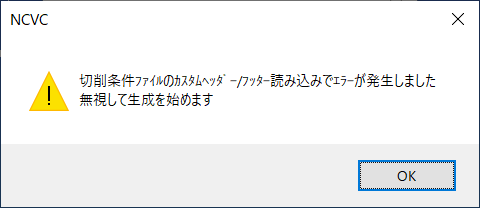
\includegraphics{No1/fig/error.png}
\caption{カスタムファイルのエラーメッセージ}
\label{fig:error.png}
\end{figure}

\newpage

\end{document}
